\section{Trusts}
\label{active-directory:trust}


A trust relationship (also called a trust) is a logical relationship established between domains to allow authentication and authorization to shared resources. The authentication process verifies the identity of the user, and the authorization process determines what the user is permitted to do on a computer system or network. Once a user requesting access to a resource computer in another domain has been authenticated by the resource domain, the resource computer compares the user’s credentials to the permissions assigned within its security descriptor to help determine the user’s level of authorization to that resource. A security descriptor contains access control lists (ACLs) that identify the users and groups that are assigned or denied access permissions on a resource.

In its simplest form, a trust acts as a technological drawbridge, by either allowing or disallowing authentication traffic to flow between two or more domains. When a trust relationship is created between two domains, traffic is allowed over the bridge, permitting the sharing of resources between them, as shown in the following illustration.

An Active Directory (AD) Forest is the security and administrative boundary for
objects and entities.
\href{https://social.technet.microsoft.com/wiki/contents/articles/50969.active-directory-forest-trust-attention-points.aspx}{trust}
is used to establish \verb+forest-forest+ or \verb+domain-domain+
authentication, allowing users to access resources in (or administer)  another
domain outside of the domain their account resides in. A trust  creates a link
between the authentication systems of two domains.

Often, domain trusts are set up improperly and provide unintended  attack
paths. Also, trusts set up for ease of use may not be reviewed  later for
potential security implications. Mergers and acquisitions can  result in
bidirectional trusts with acquired companies, unknowingly  introducing risk
into the acquiring company's environment. It is not  uncommon to be able to perform an attack such as Kerberoasting against a  domain outside the principal domain and obtain a user that has  administrative access within the principal domain.


\subsection{Trust Paths}
The direction that a trust is assigned determines the trust path used for authentication. A trust path is defined by the series of trust relationships that authentication requests must follow between domains.

Before a user can access a resource in another domain, the security system on domain controllers must determine whether the trusting domain has a trust relationship with the trusted domain. To determine this, the security system computes the trust path between a domain controller in the trusting domain and a domain controller in the trusted domain.

\subsection{Trusted Domain Object}
Each domain or forest trust within an organization is represented by a Trusted Domain Object (TDO) stored in the System container within its domain.

\begin{itemize}
    \item domain trust TDO store:
        \begin{itemize}
            \item  DNS domain name,
            \item domain SID
            \item trust type
            \item trst transitivity
            \item the reciprocal domain name
        \end{itemize}
    \item Forest trust TDOs store in addition (to identify all of the trusted namespaces from the partner forest)
        \begin{itemize}
            \item domain tree names
            \item UPN suffixes
            \item SPN suffixes
            \item SID namespaces
        \end{itemize}
\end{itemize}


\begin{itemize}
    \item 
        All domains in a forest have knowledge of the trust relationships that are in place throughout the forest
    \item 
        when two or more forests are joined together through forest trusts, the forest root domains in each forest have knowledge of the trust relationships that are in place throughout all of the domains in trusted forests
\end{itemize}

Both domains in a trust relationship share a password, which is stored in the TDO object in Active Directory. As part of the account maintenance process, every thirty days, the trusting domain controller changes the password stored in the TDO.


\subsection{Trust Flow}
\subsubsection{One-Way and Two-Way Trusts}

\subsubsection{Transitive and Nontransitive Trusts}

\subsection{Trust Types}
The types of domains included in the trust relationship affect the type of trust that is created.
\begin{itemize}
    \item Two types of trusts are created automatically when a new domain is added to a domain tree or forest root domain
        \begin{itemize}
            \item Parent-child trust
            \item Tree-root trust
        \end{itemize}
    \item Four other types of trusts can be manually created
\end{itemize}

\begin{figure}
  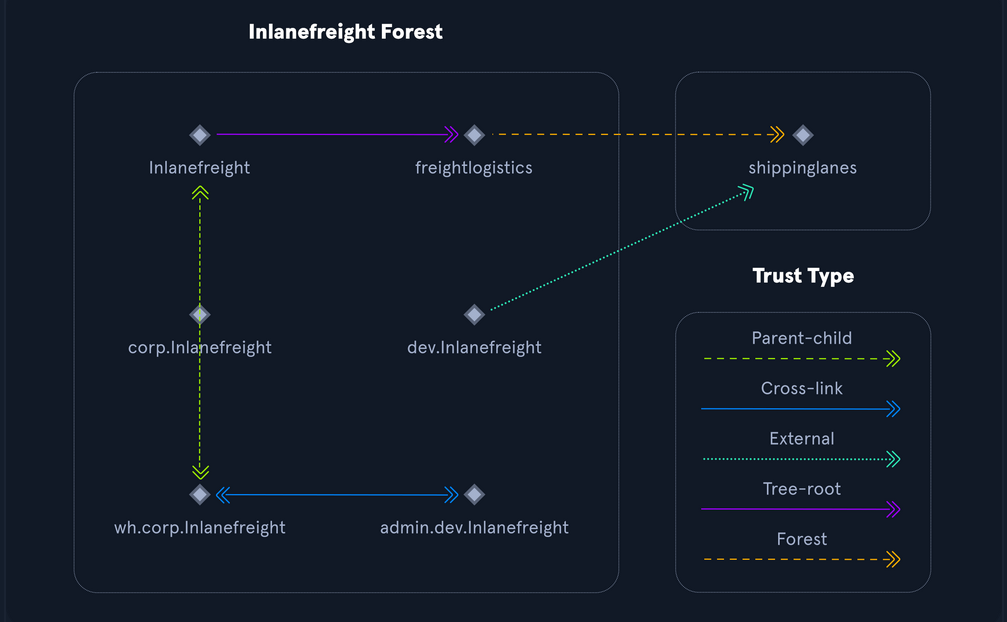
\includegraphics[width=\linewidth]{ad/knowledge/images/trusts.png}
  \caption{AD trusts}
  \label{fig:ad-trusts}
\end{figure}

\subsubsection{Parent-child trust}
whenever a new domain is created in a tree:
\begin{itemize}
    \item It can exist only between two domains in the same tree and namespace.
    \item The parent domain is always trusted by the child domain
    \item transitive and two-way (to allow the GC replication)
\end{itemize}

\subsubsection{Tree-root trust}
stablished when you add a new domain tree to a forest:
\begin{itemize}
    \item stablished only between the roots of two trees in the same forest
    \item transitive and two-way
\end{itemize}

\subsubsection{Shortcut (cross-link) Trusts}
A one-way or two-way transitive trusts between child domain to speed up authentication.


\subsubsection{External Trusts}
A trust relationship created between Active Directory domains that are in different forests.

i{\bf External trusts provide access to resources in a domain outside of the forest that is not already joined by a forest trust}

An external trust relationship has the following characteristics:
\begin{itemize}
    \item 
    It is nontransitive.

    \item 
    It must be established manually in each direction to create a two-way external trust relationship. 
    \item 
    It enforces SID filter quarantining by default. External trusts created from the trusting domain use SID filter quarantining to verify that incoming authentication requests made from security principals in the trusted domain contain only SIDs of security principals in the trusted domain. SID filter quarantining ensures that any misuse of the SID history attribute on security principals (including inetOrgPerson) in the trusted forest cannot pose a threat to the integrity of the trusting forest.
\end{itemize}

When a trust is established between a domain in a forest and a domain outside of that forest, security principals from the external domain can access resources in the internal domain. Active Directory creates a {\bf foreign security principal object} in the internal domain to represent each security principal from the trusted external domain. These foreign security principals can become members of domain local groups in the internal domain. Directory objects for foreign security principals are created by Active Directory and should not be manually modified. You can view foreign security principal objects from Active Directory Users and Computers by enabling advanced features.


\subsubsection{Forest Trusts}
a transitive trust between one forest root domain and another forest root domain. Forest trusts also enforce SID filtering


\subsubsection{Realm (MIT) Trusts}
A trust relationship can be established with a non-Windows Kerberos realm



\begin{figure}
  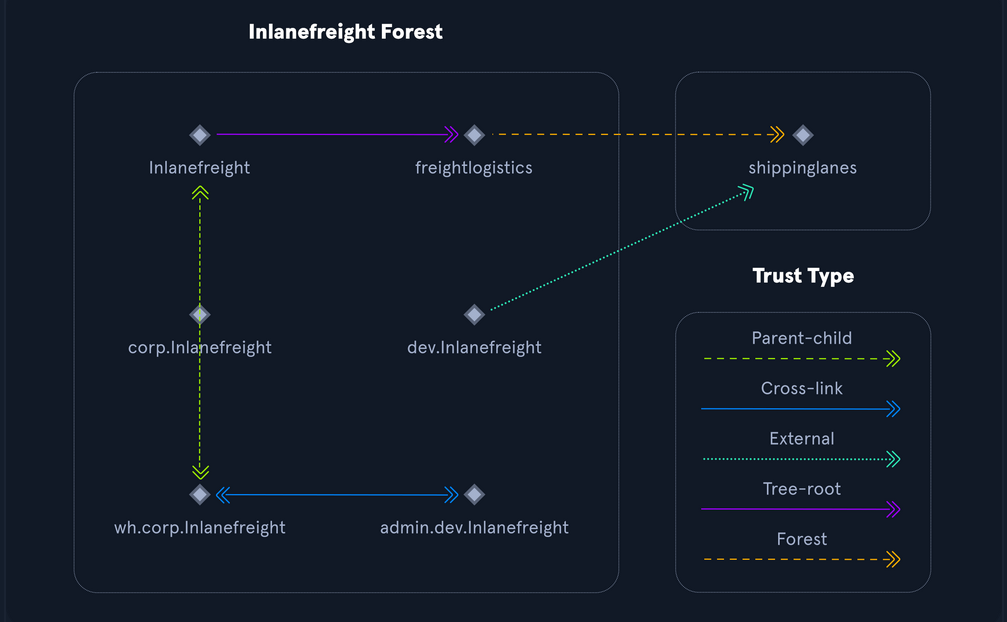
\includegraphics[width=\linewidth]{ad/knowledge/images/trusts.png}
  \caption{AD trusts}
  \label{fig:ad-trusts}
\end{figure}




\subsection{Overview of Authentication Referral Processing}
This section describes the processes and interactions that occur as resources are accessed across trusts and authentication referrals are evaluated.

When a request for authentication is referred to a domain, the domain controller in that domain must determine whether a trust relationship exists with the domain from which the request comes, as well as the direction of the trust and whether the trust is transitive or nontransitive, before it authenticates the user to access resources in the domain. 

The authentication process that occurs between trusted domains varies according to the authentication protocol in use.


\subsubsection{Kerberos V5 Referral Processing}
If the client uses Kerberos V5 for authentication, it requests a ticket to the server in the target domain from a domain controller in its account domain

If the target domain is different from the current domain, the KDC follows a logical process to determine whether an authentication request can be referred:
\begin{itemize}
    \item If the current domain is trusted directly by the domain of the server that is being requested
        \begin{itemize}
            \item send the client a referral to the requested domain
        \end{itemize}
    \item else if  a transitive trust relationship exist between the current domain and the next domain on the trust path
        \begin{itemize}
            \item send the client a referral to the next domain on the trust path
        \end{itemize}
    \item else
        \begin{itemize}
            \item send the client a logon-denied message
        \end{itemize}
\end{itemize}

an {\bf referal ticket} is a TGS that includes a {\bf inter-realm TGT} which is a TGT encrypted/signed with the inter-realm trust key that the domains previously exchanged, instead of the first domain’s krbtgt account.

The foreign domain then verifies/decrypts the TGT included in the referral by decrypting it with the previously negotiated inter-realm trust key, and goes about the rest of the normal Kerberos process.


{\bf Processing of Authentication Requests Over Domain Trusts}:


{\bf Processing of Authentication Requests Over Forest Trusts}:


\subsubsection{NTLM Referral Processing}

the initial request for authentication goes directly from the client to the resource server in the target domain. 

This server creates a challenge to which the client responds.

The server then sends the user’s response to a domain controller in its computer account domain.

This domain controller checks the user account against its security accounts database. If the account does not exist in the database, the domain controller determines whether to perform pass-through authentication, forward the request, or deny the request by using the following logic:

\begin{itemize}
    \item If the current domain have a direct trust relationship with the user’s domain
        \begin{itemize}
            \item the domain controller sends the credentials of the client to a domain controller in the user’s domain for pass-through authentication
        \end{itemize}
    \item else if the current domain have a transitive trust relationship with the user’s domain
        \begin{itemize}
            \item pass the authentication request on to the next domain in the trust path. This domain controller repeats the process by checking the user’s credentials against its own security accounts database
        \end{itemize}
    \item else
        \begin{itemize}
            \item send the client a logon-denied message
        \end{itemize}
\end{itemize}


\subsubsection{Other Authentication Protocol Referral Processing}


\subsection{Network Ports used by Trusts}

see~\href{https://learn.microsoft.com/en-us/previous-versions/windows/it-pro/windows-server-2003/cc773178(v=ws.10)?redirectedfrom=MSDN#network-ports-used-by-trusts}{Network Ports used by Trusts}
